\subsection{Introduction}
To answer what User-Centred Design (UCD) is, we first need to establish what it \textit{isn't}:
\begin{itemize}
    \item UCD doesn't mean talking \textit{to} the users and asking what they want {\scriptsize (that's pretty much a user study)}
    \item UCD doesn't mean testing the usability of the design in the end
    \item UCD is not just for user interfaces or software {\scriptsize (it can also be for Programming Languages)}
    \item UCD doesn't guarantee a perfect design {\scriptsize (duh)}
\end{itemize}

So, what is it then? It is characterized by:
\begin{enumerate}
    \item \bi{An early focus on users and tasks} {\scriptsize (get a psychology degree first)}
    \item \bi{Empirical measurement} {\scriptsize (Come up with some sort of measurement of performance)}
    \item \bi{Iterative Design} {\scriptsize (Identify and fix problems)}
\end{enumerate}
That all is very obvious and the hardest part for Computer Scientists of course is the first property.
The second property is typically done via user studies, where you keep track of a lot of data on how users interact with your application.
Don't shy away from storing way more details than you think you could possibly use, it will make it much easier to evaluate things later on.
    {\tiny (Can you tell that I am speaking from experience?)}

That brings us to a formal definition from ``The Design of Everyday Things'' by Donald A. Norman (2013),
which also includes famous examples such as the \hlhref{https://www.youtube.com/watch?v=qtCEoGyfsxk}{Norman Door}.

\begin{definition}[]{User-Centred Design}
    User-Centered Design (UCD) is an iterative design process in which designers focus on the users and their needs in each phase of the design process.
    UCD involves researching user behaviors, needs, and experiences and incorporating user feedback through multiple iterations of prototyping and testing to ensure usability,
    accessibility, and satisfaction. The goal is to develop solutions that align with real user needs rather than assumptions about those needs.
\end{definition}

For property one and two, typically this is an iterating over \textit{understanding the problem}, \textit{building} and \textit{evaluating}.

The full loop looks a like this:
\begin{center}
    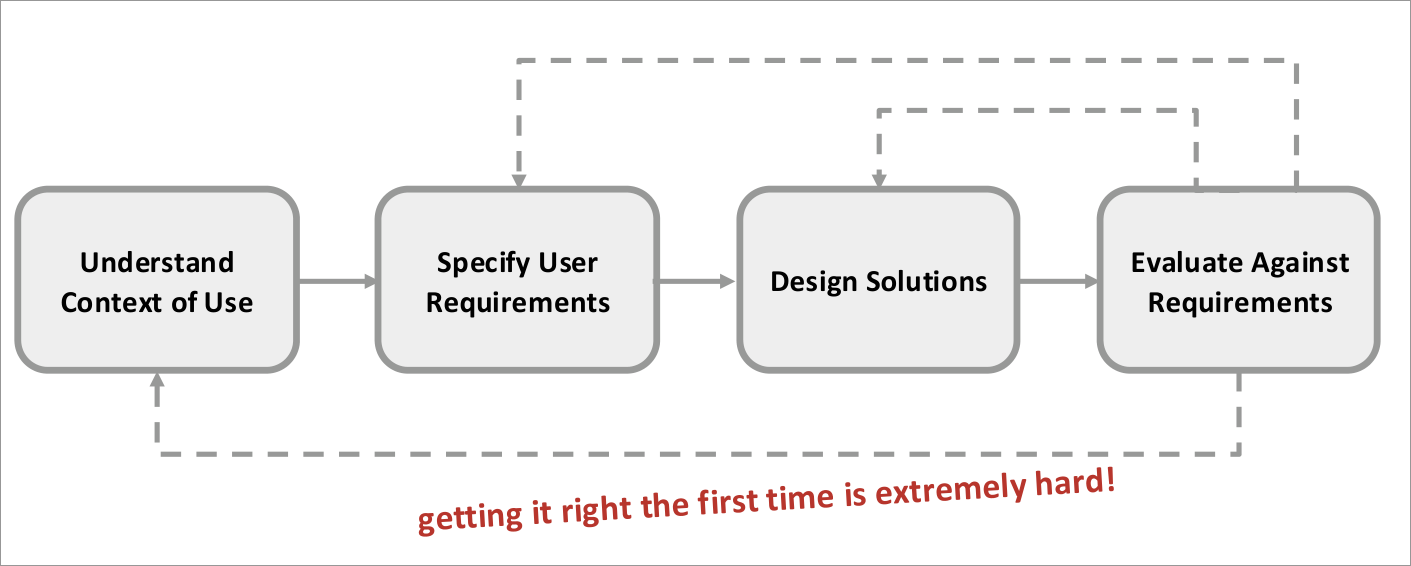
\includegraphics[width=0.7\linewidth]{assets/user-centtered-design-process.png}
\end{center}

Coming up with a good idea is hard, which is why this quote is important:

\fancyquote{The best way to have a good idea is to have \textit{lots of ideas}}{\textit{Linus Pauling}}

The only question that remains is, when are you done? See Section~\ref{sec:evaluation}
